\documentclass[../../main.tex]{subfiles}
\begin{document}

\begin{flushright}
  \footnotesize\textit{【自動文字起こし・要確認】}
\end{flushright}

[解] (1) 対称性から$a \ge 0$で考える．$C_1: y=x^2+1, C_2: y=kx^2$とする．$C_1$と$C_2$で囲まれた部分の面積$S_1$，$L$と$C_2$で囲まれた面積$S_2$とする．題意から，
\begin{figure}[htb]
  \centering
  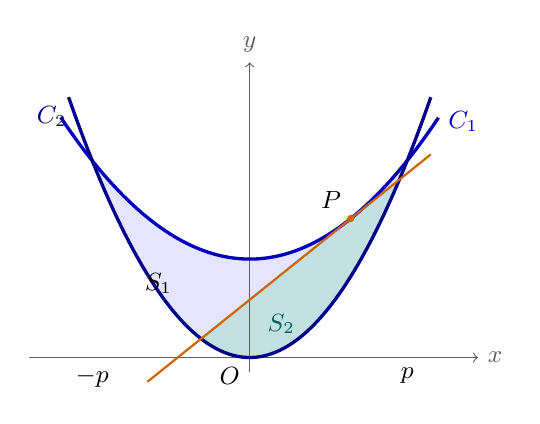
\begin{tikzpicture}[x=2.0cm,y=1.25cm,every node/.style={font=\small}]
    % 形状確認用に k=2, a=sqrt(2-cuberoot(4)) を選ぶ．
    \fill[blue!10] plot[domain=-1:1,samples=80] (\x,{\x*\x+1})
    -- plot[domain=1:-1,samples=80] (\x,{2*\x*\x}) -- cycle;
    \fill[teal!24] plot[domain=-0.299:0.941,samples=60]
    (\x,{1.284*\x+0.587})
    -- plot[domain=0.941:-0.299,samples=60] (\x,{2*\x*\x}) -- cycle;
    \draw[->,gray!75!black] (-1.4,0)--(1.45,0) node[right] {$x$};
    \draw[->,gray!75!black] (0,-0.15)--(0,3.0) node[above] {$y$};
    \draw[blue!75!black,very thick,domain=-1.2:1.2,samples=80]
    plot (\x,{\x*\x+1});
    \draw[blue!55!black,very thick,domain=-1.15:1.15,samples=80]
    plot (\x,{2*\x*\x});
    \draw[orange!80!black,thick,domain=-0.65:1.15]
    plot (\x,{1.284*\x+0.587});
    \fill[orange!80!black] (0.642,1.413) circle (1.3pt);
    \node[above left] at (0.642,1.413) {$P$};
    \node[right,blue!75!black] at (1.2,2.4) {$C_1$};
    \node[left,blue!55!black] at (-1.1,2.45) {$C_2$};
    \node at (-0.58,0.75) {$S_1$};
    \node[teal!75!black] at (0.20,0.34) {$S_2$};
    \node[below left] at (0,0) {$O$};
    \node[below] at (-1,0) {$-p$};
    \node[below] at (1,0) {$p$};
  \end{tikzpicture}
  \caption{放物線に挟まれた淡青の領域$S_1$と，橙の接線$L$より下の青緑の領域$S_2$}
\end{figure}
$$
S_1 = 2S_2 \cdots \text{\textcircled{1}}
$$
である．ここで，$p = \sqrt{\dfrac{1}{k-1}}$とすると，
$$
S_1 = \int_{-p}^p \{ x^2+1 - kx^2 \} dx
$$
$$
= \dfrac{k-1}{6} (2p)^3
$$
$$
= \dfrac{4}{3} (k-1) \left( \dfrac{1}{k-1} \right)^{\frac{3}{2}} \cdots \text{\textcircled{2}}
$$
で，又，$L: y = f(x) = 2ax - a^2 + 1$から，$f(x) = kx^2$の2解$\alpha, \beta \ (\alpha \le \beta)$として，
$$
S_2 = \int_\alpha^\beta \{ f(x) - kx^2 \} dx = \dfrac{k}{6}(\beta-\alpha)^3 \cdots \text{\textcircled{3}}
$$
となる．$\alpha \le \beta$から，
$$
\beta - \alpha = \dfrac{2}{k}\sqrt{(1-k)a^2+k}
$$
だから\textcircled{3}に代入して，
$$
S_2 = \dfrac{k}{6} \left( \dfrac{2}{k} \right)^3 \left\{ (1-k)a^2+k \right\}^{\frac{3}{2}}
$$
$$
= \dfrac{4}{3}\dfrac{1}{k^2} \left\{ (1-k)a^2+k \right\}^{\frac{3}{2}} \cdots \text{\textcircled{4}}
$$
\textcircled{1}, \textcircled{2}, \textcircled{4}から
$$
(k-1)\left(\dfrac{1}{k-1}\right)^{\frac{3}{2}} = \dfrac{2}{k^2} \left\{ (1-k)a^2+k \right\}^{\frac{3}{2}}
$$
両辺0以上から，2/3乗して，
$$
\left(\dfrac{1}{k-1}\right)^{\frac{1}{2}} = \left(\dfrac{2}{k^2}\right)^{\frac{2}{3}} \{ (1-k)a^2+k \}
$$
$$
\therefore a^2 = - \dfrac{ \left(\dfrac{k^4}{4(k-1)}\right)^{\frac{1}{3}} - k }{k-1}
$$

\paragraph{(2)}
$$
a^2 = - \left\{ \dfrac{k^4}{4(k-1)^4} \right\}^{\frac{1}{3}} + \dfrac{k}{k-1}
$$
$$
= - \left( \dfrac{1}{4} \right)^{\frac{1}{3}} \left( \dfrac{1}{1-1/k} \right)^{\frac{4}{3}} + \dfrac{1}{1-1/k}
$$
$$
\longrightarrow 1 - \left( \dfrac{1}{4} \right)^{\frac{1}{3}} \quad (k \to +\infty)
$$

\end{document}
